
% When you want to compile, run these 4 steps in order.
% xelatex LabReport_name.tex
% bibtex LabReport_name
% xelatex LabReport_name.tex
% xelatex LabReport_name.tex

\documentclass[openany, a4paper, 12pt]{book}
\usepackage{multicol} % 柔軟に二段組を使いたい場合に便利

% import packages
\usepackage[pdfborder={0 0 0}, colorlinks=false]{hyperref} 
\usepackage{graphicx}
\usepackage{xeCJK}
\usepackage[font=small,labelfont=bf]{caption} 
\usepackage{subcaption}
\usepackage[a4paper, margin=2.5cm]{geometry}
\usepackage{hyperref}
\usepackage{setspace}
\usepackage{fancyhdr}
\usepackage{float}
\usepackage{fontspec}  
\usepackage{booktabs}  
\usepackage{placeins}
\usepackage[version=4]{mhchem}

% reference settings
\usepackage{etoolbox}
\renewcommand{\bibname}{References}
\patchcmd{\thebibliography}{\chapter*{\bibname}}{\section*{\bibname}}{}{}
\addcontentsline{toc}{section}{References}

% chapter settings
\renewcommand{\thesection}{\arabic{section}}
\renewcommand{\thesubsection}{\thesection.\arabic{subsection}}
\renewcommand{\thesubsubsection}{\thesubsection.\arabic{subsubsection}}
\setcounter{tocdepth}{2} % section + subsection まで表示
\setcounter{secnumdepth}{3} % subsubsection まで番号付け

% ToC settings
\usepackage{tocloft} 
\setlength{\cftbeforesecskip}{4pt}      % section margin
\setlength{\cftbeforesubsecskip}{2pt}   % subsection margin
% List of figures
\renewcommand{\cftfigpresnum}{Figure~}  
\renewcommand{\cftfignumwidth}{7em}     
% List of tables
\renewcommand{\cfttabpresnum}{Table~}   
\renewcommand{\cfttabnumwidth}{7em}    

\usepackage[justification=raggedright,singlelinecheck=false]{caption} 
\pagestyle{plain}

% -----------------------------------------------------

% title of the course
\newcommand{\etitle}{Introduction into studying fatty acid and lipid metabolism}
\setmainfont{Times New Roman} % font

\begin{document}
% --- タイトルページなどは一段 ---
\onecolumn 
\thispagestyle{empty}

\setmainfont{Times New Roman}

%\pagenumbering{gobble}  % ページ番号を表示しない

\vspace*{2cm}
\begin{center}
    {\LARGE \textbf{Laboratory Report}}\\[1em]
    Quantitative Biology Week I
\end{center}

\vspace*{4cm}

\begin{center}
    \LARGE \textbf{title of the course}\\[0.5em]
\end{center}

\vfill

\begin{center}
    Your Name\\
    Matr.-Nr.: 1111111111\\[1em]
    Heidelberg University\\
    your.name@stud.uni-heidelberg.de
\end{center}


\setcounter{page}{1}  % page count starts from 1
\pagestyle{plain}
\section*{Abstract}

\begin{minipage}{\linewidth}
\centering
\begin{large}
\begin{tabular}{|p{0.97\linewidth}|}
\hline
\etitle \\ \hline
\end{tabular}
\end{large}
\end{minipage}
Caption caption caption caption caption caption caption caption caption caption caption caption caption caption caption caption caption caption caption caption caption caption caption caption caption caption caption caption caption caption caption caption caption caption caption caption caption caption caption caption caption caption caption caption caption caption caption caption caption caption caption caption caption caption caption caption caption caption caption caption caption caption caption caption caption caption caption caption caption caption caption caption caption caption caption caption caption caption caption caption caption caption caption caption caption caption caption caption caption caption caption caption caption caption caption caption caption caption caption caption caption caption caption caption caption caption caption caption caption caption caption caption caption caption. 
\vspace{0.5em}


\tableofcontents
% \clearpage
% \listoffigures   % 図の一覧（List of Figures）
% \listoftables    % 表の一覧（List of Tables）
% \clearpage

\section{Introduction}
\subsection{section}
Caption caption caption caption caption caption caption caption caption caption caption caption caption caption caption caption caption caption caption caption caption caption caption caption caption caption caption caption caption caption \cite{parkhi2012cats}. 

% -----------------------------------------------------

\subsection{section}
 caption caption caption caption caption caption caption caption caption caption caption caption caption caption caption caption caption caption caption caption caption caption caption caption caption caption caption caption caption caption caption caption caption caption caption caption caption caption caption caption caption caption caption caption caption caption caption caption caption caption caption caption caption caption caption caption caption caption caption caption
\section{Method}
\subsection{Cell culture}
Caption caption caption caption caption caption caption caption caption caption caption caption caption caption caption caption caption caption caption caption caption caption caption caption caption caption caption caption caption caption Caption caption caption caption caption caption caption caption caption caption caption caption caption caption caption caption caption caption caption caption caption caption caption caption caption caption caption caption caption caption

% -----------------------------------------------------

\subsection{Sample preparation}
Caption caption caption caption caption caption caption caption caption caption caption caption caption caption caption caption caption caption caption caption caption caption caption caption caption caption caption caption caption caption(Fig.~\ref{fig:fig1}). CCaption caption caption caption caption caption caption caption caption caption caption caption caption caption caption caption caption caption caption caption caption caption caption caption caption caption caption caption caption caption

\begin{figure}[htbp]
    \centering
    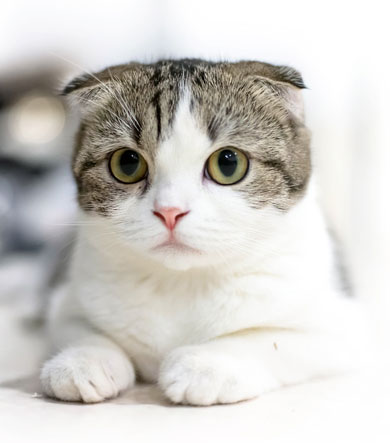
\includegraphics[width=1.0\textwidth]{figs/fig1.png}
    \caption{
        \textbf{Figure title here.}
        \\
        3Caption caption caption caption caption caption caption caption caption caption caption caption caption caption caption caption caption caption caption caption caption caption caption caption. 
    }
    \label{fig:fig1}
\end{figure}

% -----------------------------------------------------

\par
\chapter{Result}

\section{section}
Caption caption caption caption caption caption caption caption caption caption caption caption caption caption caption caption caption caption caption caption caption caption caption caption caption caption caption caption caption caption(Fig.~\ref{fig:fig2}). Caption caption caption caption caption caption caption caption caption caption caption caption caption caption caption caption caption caption caption caption caption caption caption caption caption caption caption caption caption caption caption caption caption caption caption caption caption caption caption caption caption caption caption caption caption caption caption caption caption caption caption caption caption caption caption caption caption caption caption caption caption caption caption caption caption caption caption caption caption caption caption caption caption caption caption caption caption caption caption caption caption caption caption caption caption caption caption caption caption caption caption caption caption caption caption caption caption caption caption caption caption caption caption caption caption caption caption caption caption caption caption caption caption caption. 

\begin{figure}[htbp]
    \centering
    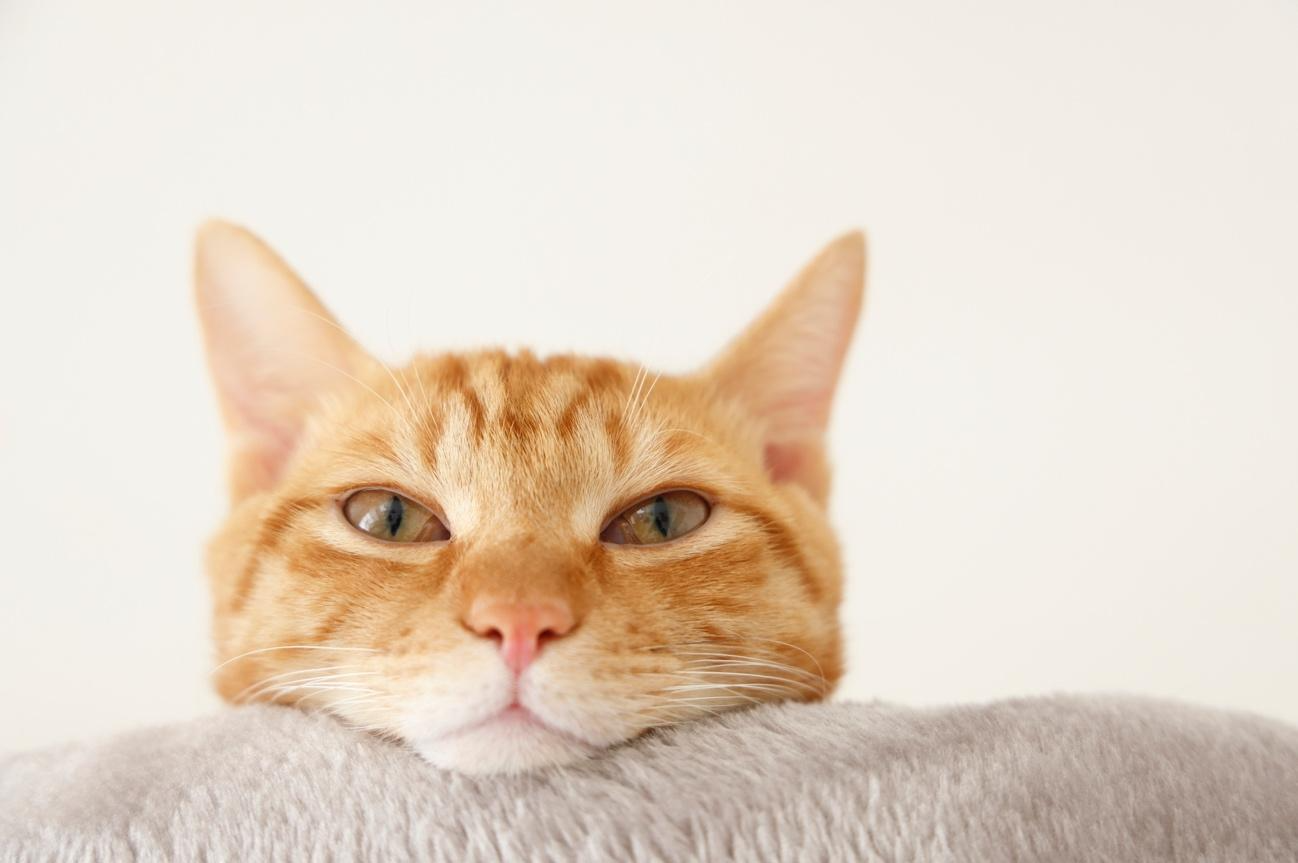
\includegraphics[width=1.0\textwidth]{figs/fig2.png}
    \caption{
        \textbf{Figure title here.}
        \\
        3Caption caption caption caption caption caption caption caption caption caption caption caption caption caption caption caption caption caption caption caption caption caption caption caption. 
    }
    \label{fig:fig2}
\end{figure}

% -----------------------------------------------------

\section{Discussion}

\subsection{section}
Caption caption caption caption caption caption caption caption caption caption caption caption caption caption caption caption caption caption caption caption caption caption caption caption caption caption caption caption caption caption caption caption caption caption caption caption caption caption caption caption caption caption caption caption caption caption caption caption caption caption caption caption caption caption caption caption caption caption caption caption caption caption caption caption caption caption caption caption caption caption caption caption caption caption caption caption caption caption caption caption caption caption caption caption caption caption caption caption caption caption caption caption caption caption caption caption caption caption caption caption caption caption caption caption caption caption caption caption caption caption caption caption caption caption. \cite{davila2018consensus}

% -----------------------------------------------------

\subsection{section}
Caption caption caption caption caption caption caption caption caption caption caption caption caption caption caption caption caption caption caption caption caption caption caption caption caption caption caption caption caption caption caption caption caption caption caption caption caption caption caption caption caption caption caption caption caption caption caption caption caption caption caption caption caption caption caption caption caption caption caption caption caption caption caption caption caption caption caption caption caption caption caption caption caption caption caption caption caption caption caption caption caption caption caption caption caption caption caption caption caption caption caption caption caption caption caption caption caption caption caption caption caption caption caption caption caption caption caption caption caption caption caption caption caption caption. Caption caption caption caption caption caption caption caption caption caption caption caption caption caption caption caption caption caption caption caption caption caption caption caption caption caption caption caption caption caption caption caption caption caption caption caption caption caption caption caption caption caption caption caption caption caption caption caption caption caption caption caption caption caption caption caption caption caption caption caption caption caption caption caption caption caption caption caption caption caption caption caption caption caption caption caption caption caption caption caption caption caption caption caption caption caption caption caption caption caption caption caption caption caption caption caption caption caption caption caption caption caption caption caption caption caption caption caption caption caption caption caption caption caption. Caption caption caption caption caption caption caption caption caption caption caption caption caption caption caption caption caption caption caption caption caption caption caption caption caption caption caption caption caption caption caption caption caption caption caption caption caption caption caption caption caption caption caption caption caption caption caption caption caption caption caption caption caption caption caption caption caption caption caption caption caption caption caption caption caption caption caption caption caption caption caption caption caption caption caption caption caption caption caption caption caption caption caption caption caption caption caption caption caption caption caption caption caption caption caption caption caption caption caption caption caption caption caption caption caption caption caption caption caption caption caption caption caption caption. 


\bibliographystyle{unsrt}
\bibliography{ref.bib}
\input{appendix}

\end{document}


